\section{实验验证}

本章介绍实验部分。第一节为实验平台软硬件配置。第二节介绍LLM模型与数据集选取,以及实验参数设置。第三节针对基于开销感知的内存优化策略,进行吞吐率测试。第四节针对基于公平性的用户请求调度策略,进行实时性测试。第五节分析张量交换与张量重算预测误差。第六节进行开销测试。

\subsection{实验环境}

本文开展实验使用的服务器软硬件配置如表\ref{Table:实验平台的软硬件配置}所示。使用Intel(R) Xeon(R) CPU和NVIDIA A800 80GB GPU作为硬件环境,使用CUDA-11.8、PyTorch-2.0.l、Ray2.7.1以及vLLM-0.2.5作为底层框架进行开发。服务器使用PCIe连接实现GPU-CPU通信。

\begin{table}[H]
  \centering
  \caption{实验平台的软硬件配置}
  \label{Table:实验平台的软硬件配置}
  \renewcommand{\arraystretch}{1.25}
  \small
  \begin{tabular}{c c}
    \toprule
    \textbf{软件/硬件} & \textbf{型号/版本} \\ 
    \midrule
    CPU & Intel(R) Xeon(R) CPU @ 2.60GHz  \\ 
    GPU & NVIDIA A800 PCIE 80GB \\ 
    OS & CentOS Linux 7 (Core) \\ 
    CUDA & 11.8 \\ 
    PyTorch & 2.0.1 \\ 
    Ray & 2.7.1 \\
    vLLM & 0.2.5 \\ 
    \bottomrule
  \end{tabular}
\end{table}

\subsection{模型与数据集}

本文选用OPT~\cite{OPT}(OPT-13B、OPT-30B)和Llama~\cite{Llama}(Llama-13B、Llama-32.5B)作为实验模型,在三个常见数据集(Chatbot~\cite{Chatbot}、Alpaca~\cite{Alpaca}、Summary~\cite{Summary})上进行测试。数据集信息如表\ref{Table:实验数据集选取}所示。

\begin{table}[H]
  \centering
  \caption{实验数据集选取}
  \label{Table:实验数据集选取}
  \renewcommand{\arraystretch}{1.25}
  \small
  \begin{tabular}{c c c c}
    \toprule
    \textbf{数据集} & \textbf{样本总数} & \textbf{平均输入长度} & \textbf{任务类型} \\
    \midrule
    Chatbot & 258064 & 17.02 & 对话类 \\
    Alpaca & 68912 & 19.66 & 指令类 \\
    Summary & 1799 & 340.48 & 摘要类 \\
    \bottomrule
  \end{tabular}
\end{table}

\begin{figure}[!htbp]
  \centering
  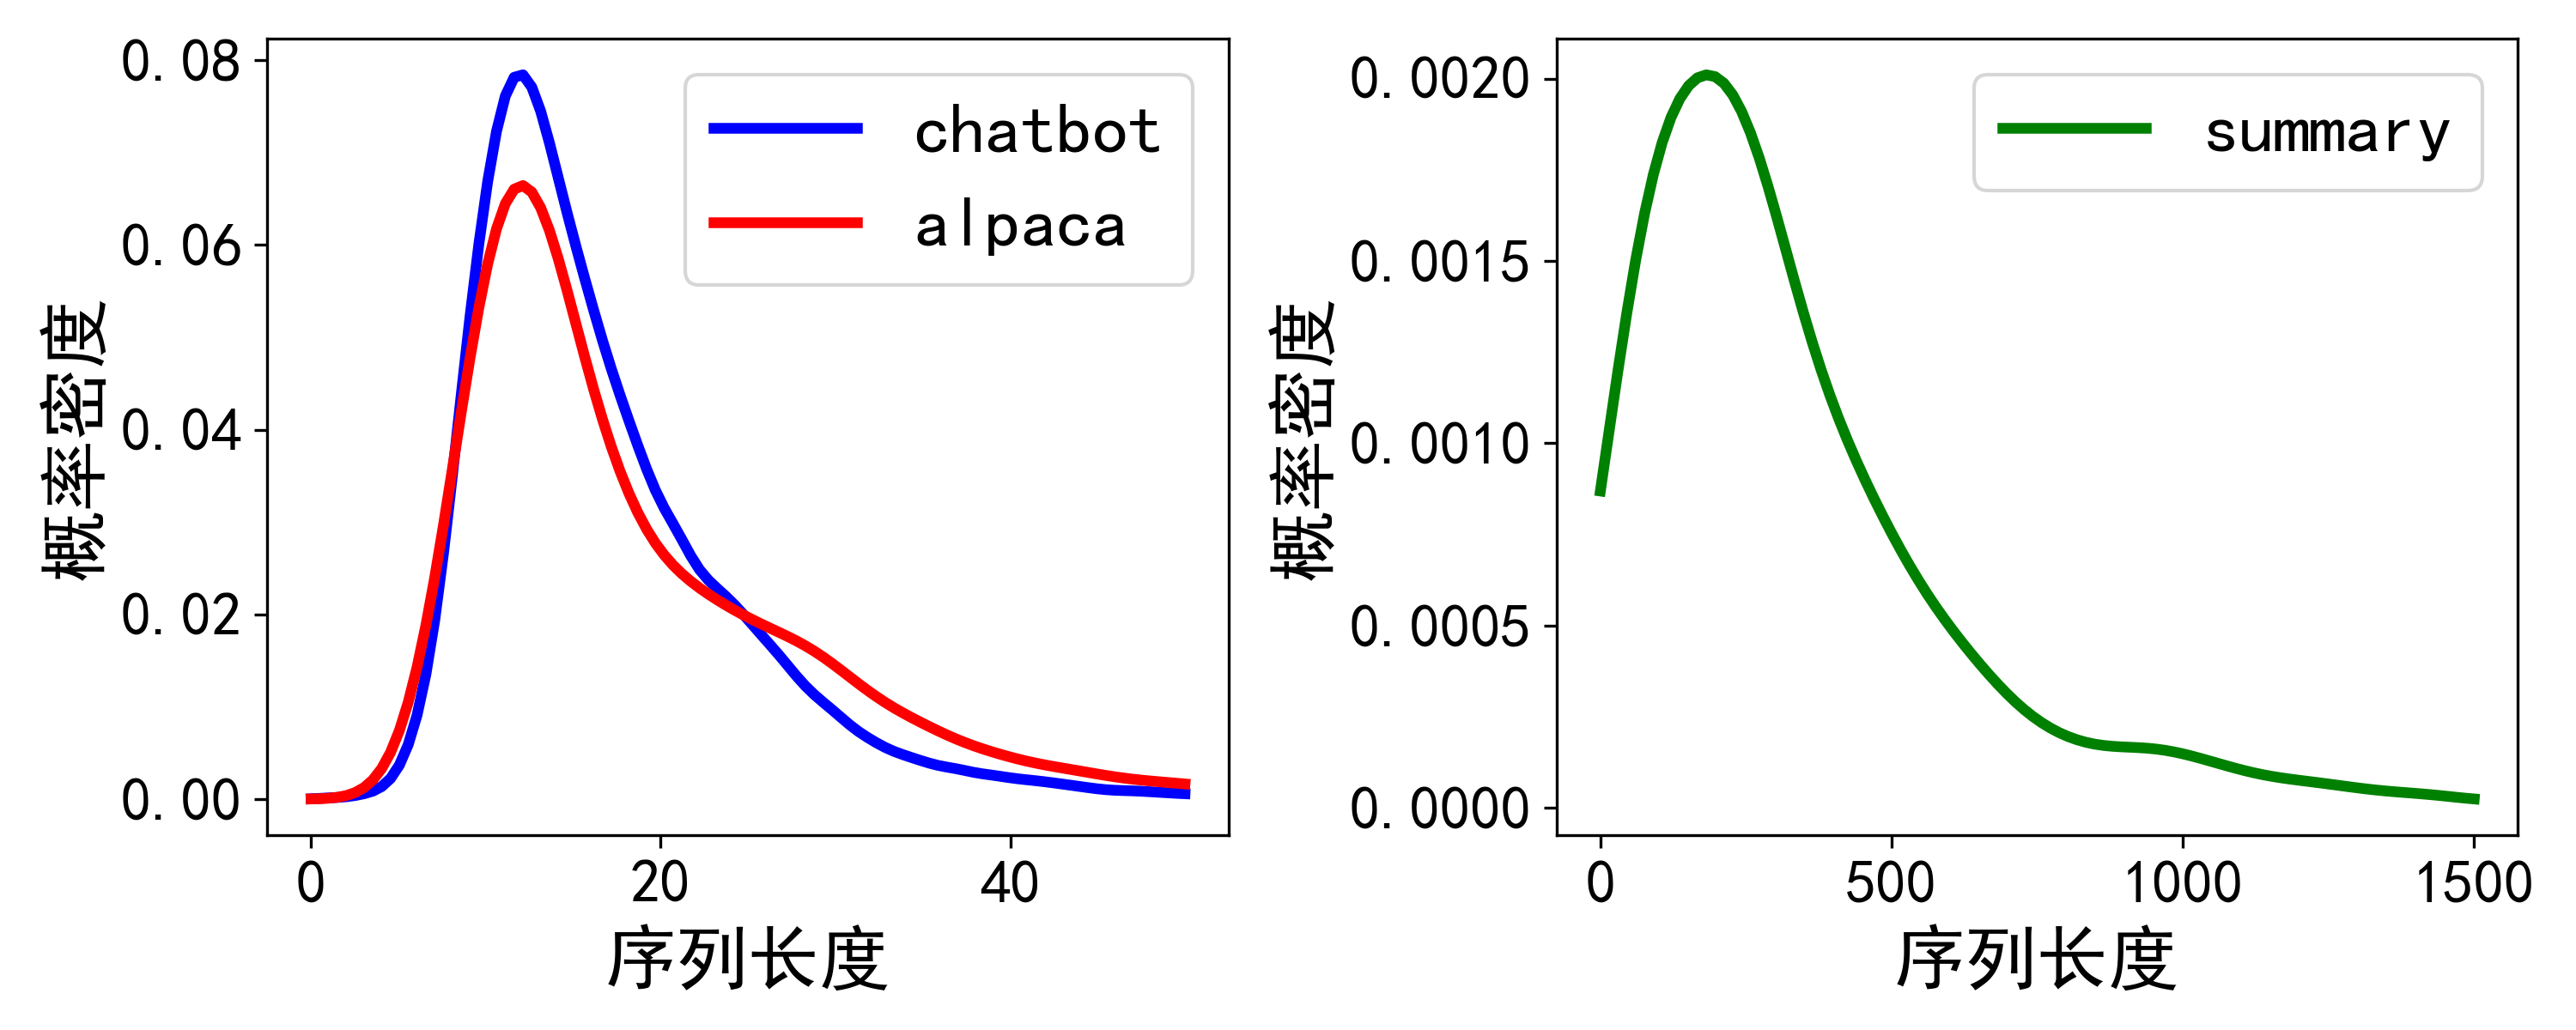
\includegraphics[width=0.9\linewidth]{序列长度分布曲线.png}
  \caption{序列长度分布曲线}
  \label{Fig:序列长度分布曲线}
\end{figure}

三个数据集的样本序列长度分布曲线如图\ref{Fig:序列长度分布曲线}所示。Chatbot和Alpaca中大多数序列长度较短,而Summary中序列长度展现出很大差异性,且包含长序列。它们涵盖了LLM应用程序面临的大部分场景。

实验过程中,将GPU内存与CPU内存使用率限制在较低水平,触发用户请求抢占现象,以模拟LLM应用程序在多任务并发场景下的运行状态。针对12个实验组,5.3章节使用整个数据集进行吞吐率测试,5.4章节在相应数据集中使用简单随机抽样法选取1000个样本进行实时性测试。

\begin{figure*}[!htbp]
  \centering
  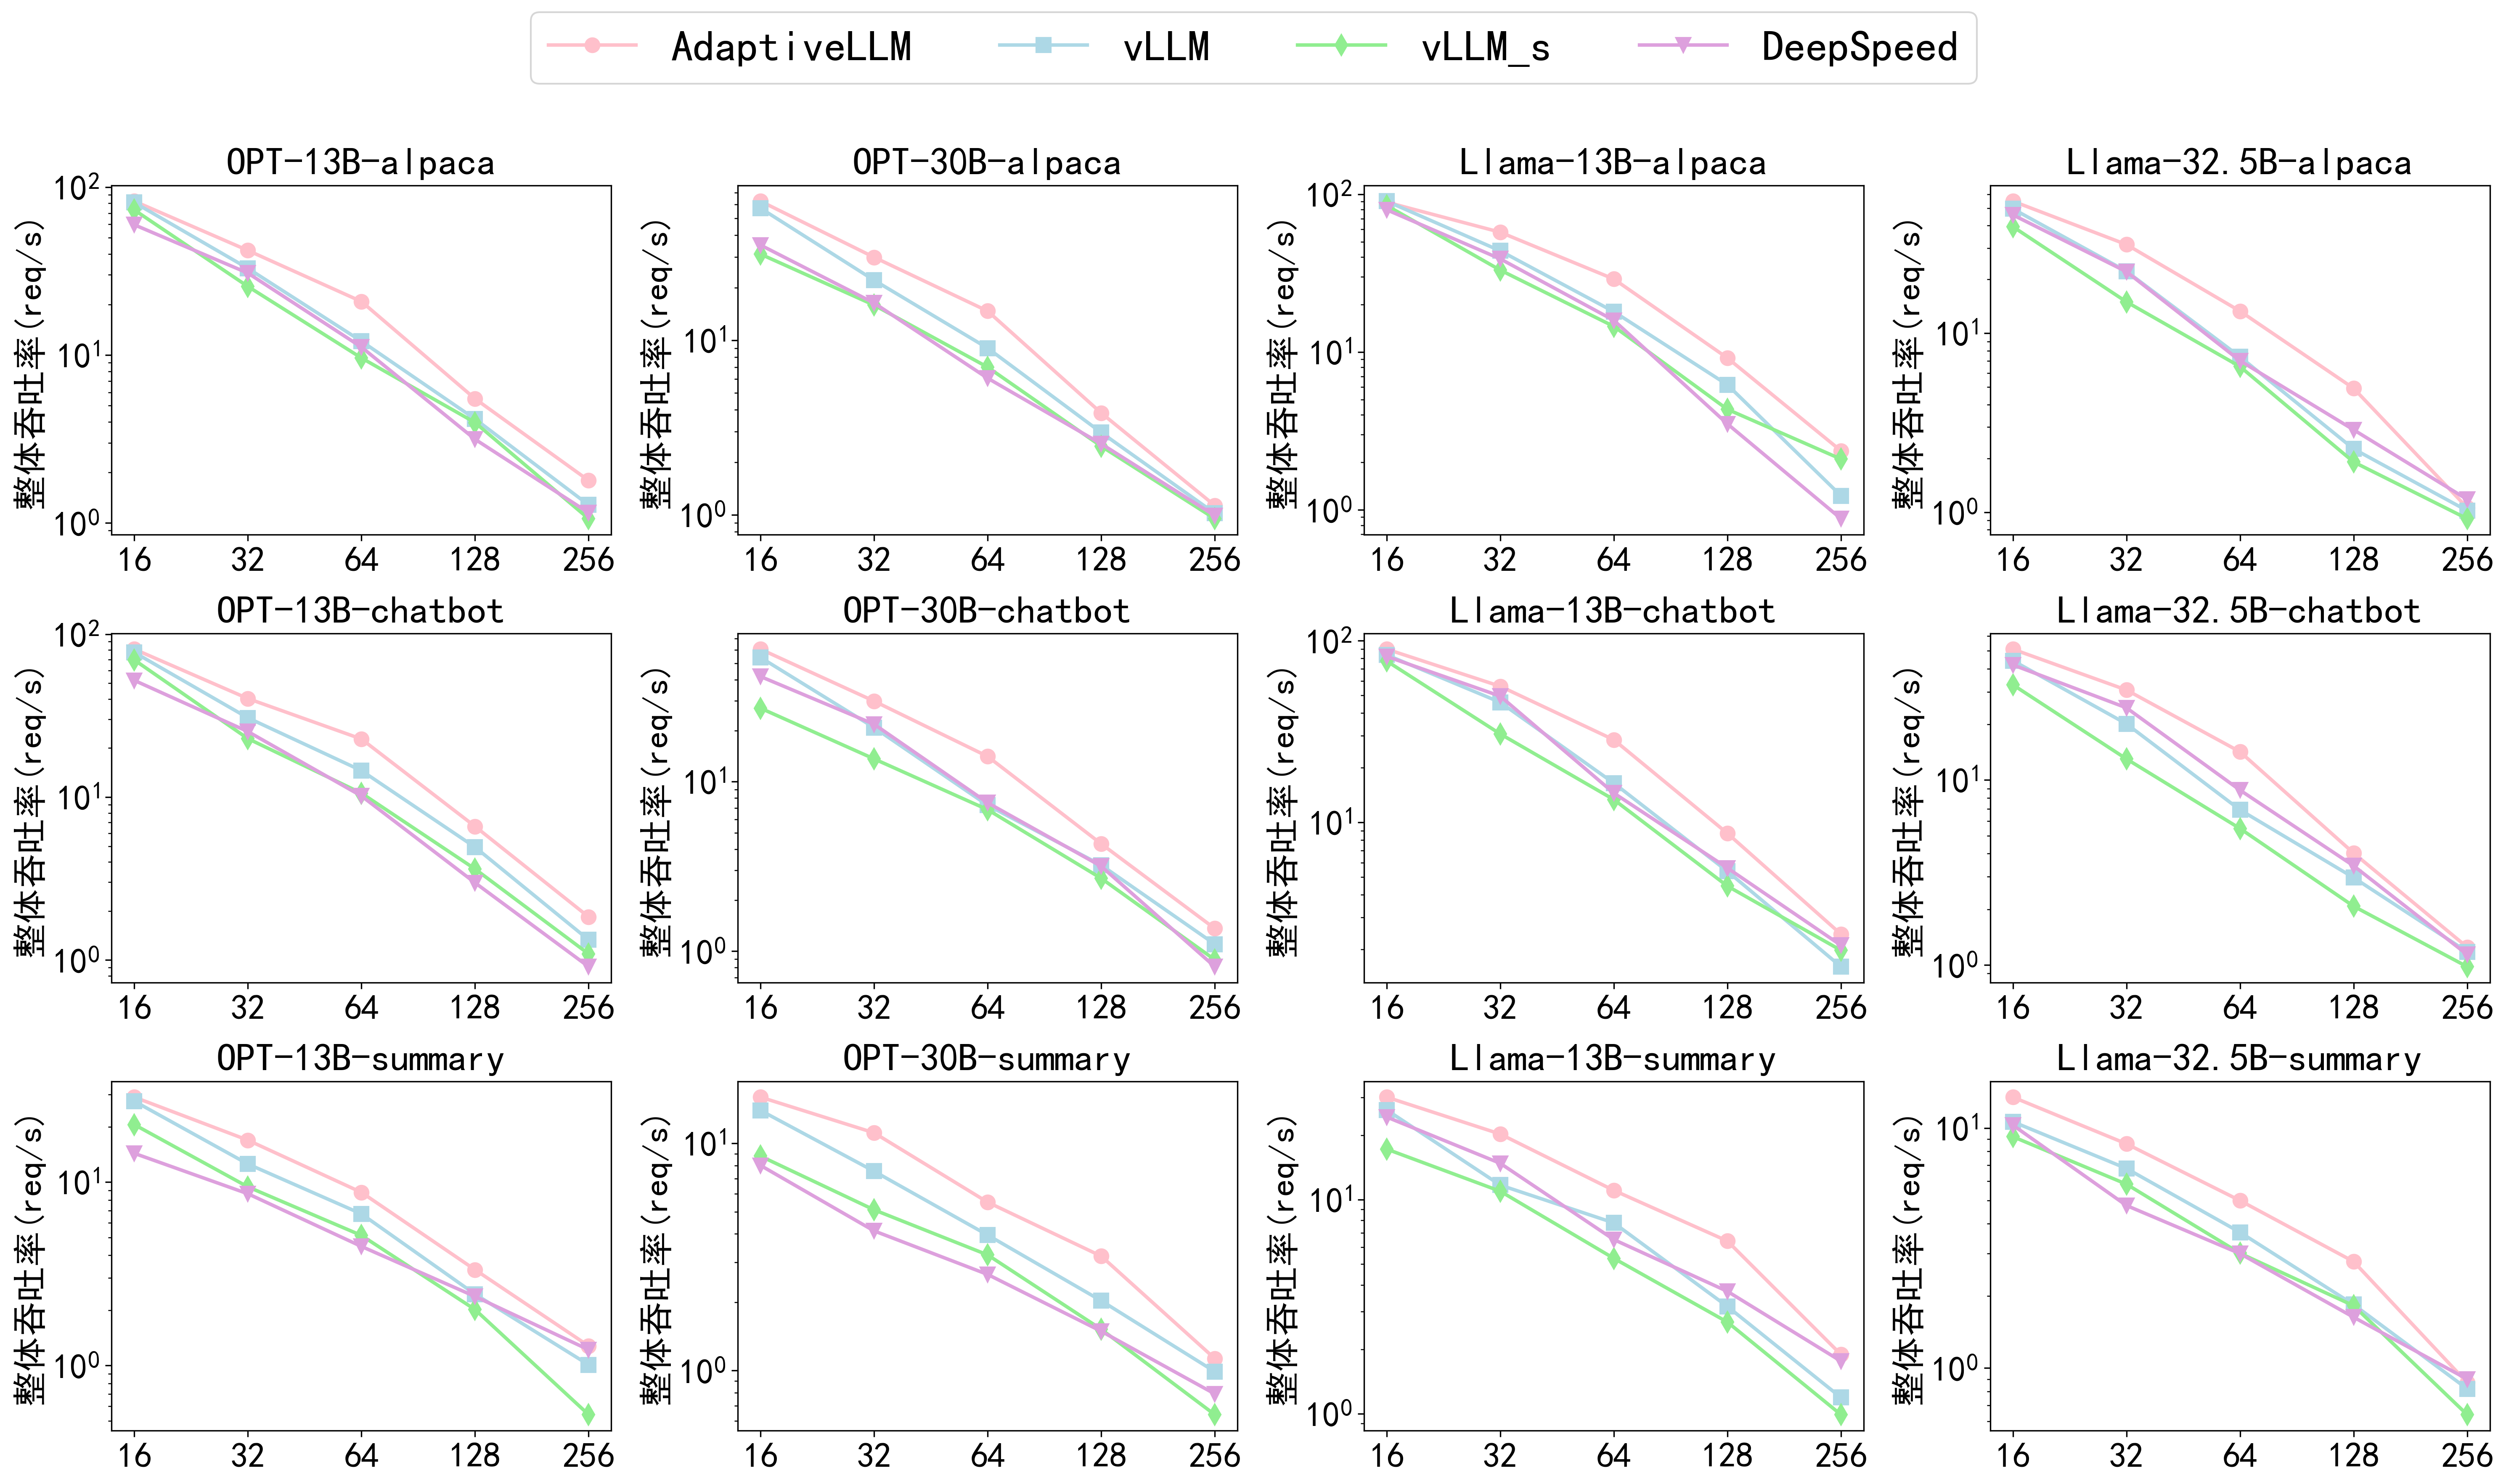
\includegraphics[width=0.9\linewidth]{整体吞吐率.png}
  \caption{推理任务吞吐率}
  \label{Fig:推理任务吞吐率}
\end{figure*}

\subsection{吞吐率测试}

本文以vLLM和DeepSpeed-MII~\cite{DeepSpeed-MII}作为基准框架,针对AdaptiveLLM进行吞吐率测试。

\begin{itemize}

  \item \textbf{vLLM:}4.4章节已经讲述,vLLM在GPU内存不足时使用单一的张量优化策略,由于本文在推理过程中使用贪心采样方式来生成新token,因此vLLM内存管理器固定调用张量重算技术。
  
  \item \textbf{vLLM$\_$s:}对vLLM框架稍加修改形成vLLM$\_$s,使其在GPU内存不足时固定调用张量交换技术。
  
  \item \textbf{DeepSpeed-MII:}DeepSpeed~\cite{DeepSpeed}是Microsoft推出的一系列LLM高效训练或推理服务框架。DeepSpeed-MII集成了分块KV Cache缓存~\cite{vLLM}、连续批处理~\cite{Continuous-Batching}、动态分割融合~\cite{DeepSpeed-FastGen}等多种LLM推理优化技术,显著降低LLM推理成本。但DeepSpeed-MII缺少对张量交换技术的支持,且在用户请求调度过程中并未考虑公平性因素。
  
\end{itemize}

\begin{table}[H]
  \centering
  \caption{AdaptiveLLM相对于基准框架的加速比}
  \label{Table:AdaptiveLLM相对于基准框架的加速比}
  \renewcommand{\arraystretch}{1.25}
  \small
  \begin{tabular}{c c c}
    \toprule
    \textbf{LLM} & \textbf{dataset} & \textbf{vLLM/vLLM\_s/DeepSpeed-MII} \\
    \midrule
    OPT-13B	& alpaca & 1.72$\times$/2.17$\times$/1.87$\times$ \\
    OPT-13B	& chatbot & 1.56$\times$/2.15$\times$/2.24$\times$ \\
    OPT-13B	& summary & 1.31$\times$/1.72$\times$/1.97$\times$ \\
    OPT-30B	& alpaca & 1.63$\times$/2.10$\times$/2.11$\times$ \\
    OPT-30B	& chatbot & 1.94$\times$/2.06$\times$/1.88$\times$ \\
    OPT-30B	& summary & 1.39$\times$/1.71$\times$/2.08$\times$ \\
    Llama-13B & alpaca & 1.61$\times$/2.00$\times$/1.83$\times$ \\
    Llama-13B & chatbot & 1.73$\times$/2.13$\times$/1.96$\times$ \\
    Llama-13B & summary & 1.42$\times$/2.08$\times$/1.70$\times$ \\
    Llama-32.5B & alpaca & 1.80$\times$/2.04$\times$/1.89$\times$ \\
    Llama-32.5B & chatbot & 2.06$\times$/2.60$\times$/1.47$\times$ \\
    Llama-32.5B & summary & 1.36$\times$/1.66$\times$/1.66$\times$ \\
    \bottomrule
  \end{tabular}
\end{table}

图\ref{Fig:推理任务吞吐率}展示了12个实验组在推理任务中的整体吞吐率测试结果,其横坐标为单序列最大输出长度。表\ref{Table:AdaptiveLLM相对于基准框架的加速比}给出了单序列最大输出长度为64时,AdaptiveLLM相对于三个基准框架的加速比。结果表明,相比于vLLM、vLLM$\_$s和DeepSpeed-MII基准框架,AdaptiveLLM实现了$1.3\times\sim2.1\times$,$1.6\times\sim2.6\times$,以及$1.4\times\sim2.3\times$的整体吞吐加速比。究其原因,在GPU内存不足时,vLLM和DeepSpeed固定调用张量重算技术,vLLM$\_$s固定调用张量交换技术,三者均无法通过预测张量交换和张量重算开销来选择更优者。若当前可使用的GPU内存较少,其性能会显著低于拥有自适应张量优化策略的AdaptiveLLM。另外,若换出的请求较多,需要考虑CPU内存不足的情况,vLLM$\_$s的批处理大小也因此被限制在较低水平。

\begin{table}[H]
  \centering
  \caption{推理任务抢占行为记录}
  \label{Table:推理任务抢占行为记录}
  \renewcommand{\arraystretch}{1.25}
  \small
  \begin{tabular}{c c c c}
    \toprule
    \textbf{LLM} & \textbf{数据集} & \textbf{重算次数} & \textbf{交换次数} \\
    \midrule
    OPT-13B & alpaca & 1464 & 91 \\
    OPT-13B & chatbot & 1441 & 87 \\
    OPT-13B & summary & 320 & 240 \\
    OPT-30B & alpaca & 1348 & 159 \\
    OPT-30B & chatbot & 1379 & 191 \\
    OPT-30B & summary & 426 & 184 \\
    Llama-13B & alpaca & 1401 & 109 \\
    Llama-13B & chatbot & 1425 & 102 \\
    Llama-13B & summary & 234 & 252 \\
    Llama-32.5B & alpaca & 1274 & 254 \\
    Llama-32.5B & chatbot & 1250 & 242 \\
    Llama-32.5B & summary & 434 & 198 \\
    \bottomrule
  \end{tabular}
\end{table}

表\ref{Table:推理任务抢占行为记录}给出了序列最大输出长度为64时,不同框架推理过程中,平均每1000个请求对应的抢占行为次数。由表可知,AdaptiveLLM可以根据模型配置,灵活选择合适的内存优化策略。当序列最大输出长度限制在较低水平时,每个请求执行推理任务所需的迭代次数较少,资源需求量低,抢占鲜有发生,此时AdaptiveLLM和vLLM性能差距不大。随着最大输出长度的增加,有限的GPU内存无法满足需求,AdaptiveLLM调用基于开销感知的内存优化策略,展现性能优势。当最大输出长度过大时,无论是AdaptiveLLM还是基准框架,其批处理大小均限制在较低水平,但AdaptiveLLM仍具有明显优势(序列最大输出长度为256时,AdaptiveLLM相比于三个基准框架实现最高1.93$\times$、2.37$\times$和2.69$\times$的加速比)。

根据预测器给出的结果可知,对于大部分短序列(如Alpaca和Chatbot数据集)而言,张量交换开销小于张量重算开销。对于大部分长序列(如Summary数据集)而言,张量交换开销大于张量重算开销。

因此,在Chatbot和Alpaca数据集中,序列长度较短,批处理大小高。随着新token的生成,GPU显存无法满足众多用户请求的KV Cache存储需求,此时大量用户请求被换出到CPU中。当CPU内存不足时,则会强制执行张量重算。

对于Summary数据集而言,序列长度较长,批处理大小低。运行请求的KV Cache内存占用量增长缓慢,导致其推理过程中抢占现象发生相对较少,不会出现CPU内存不足的情况。此时,张量重算与张量交换次数能够真实反映开销预测值的比较结果。

\begin{figure*}[!htbp]
  \centering
  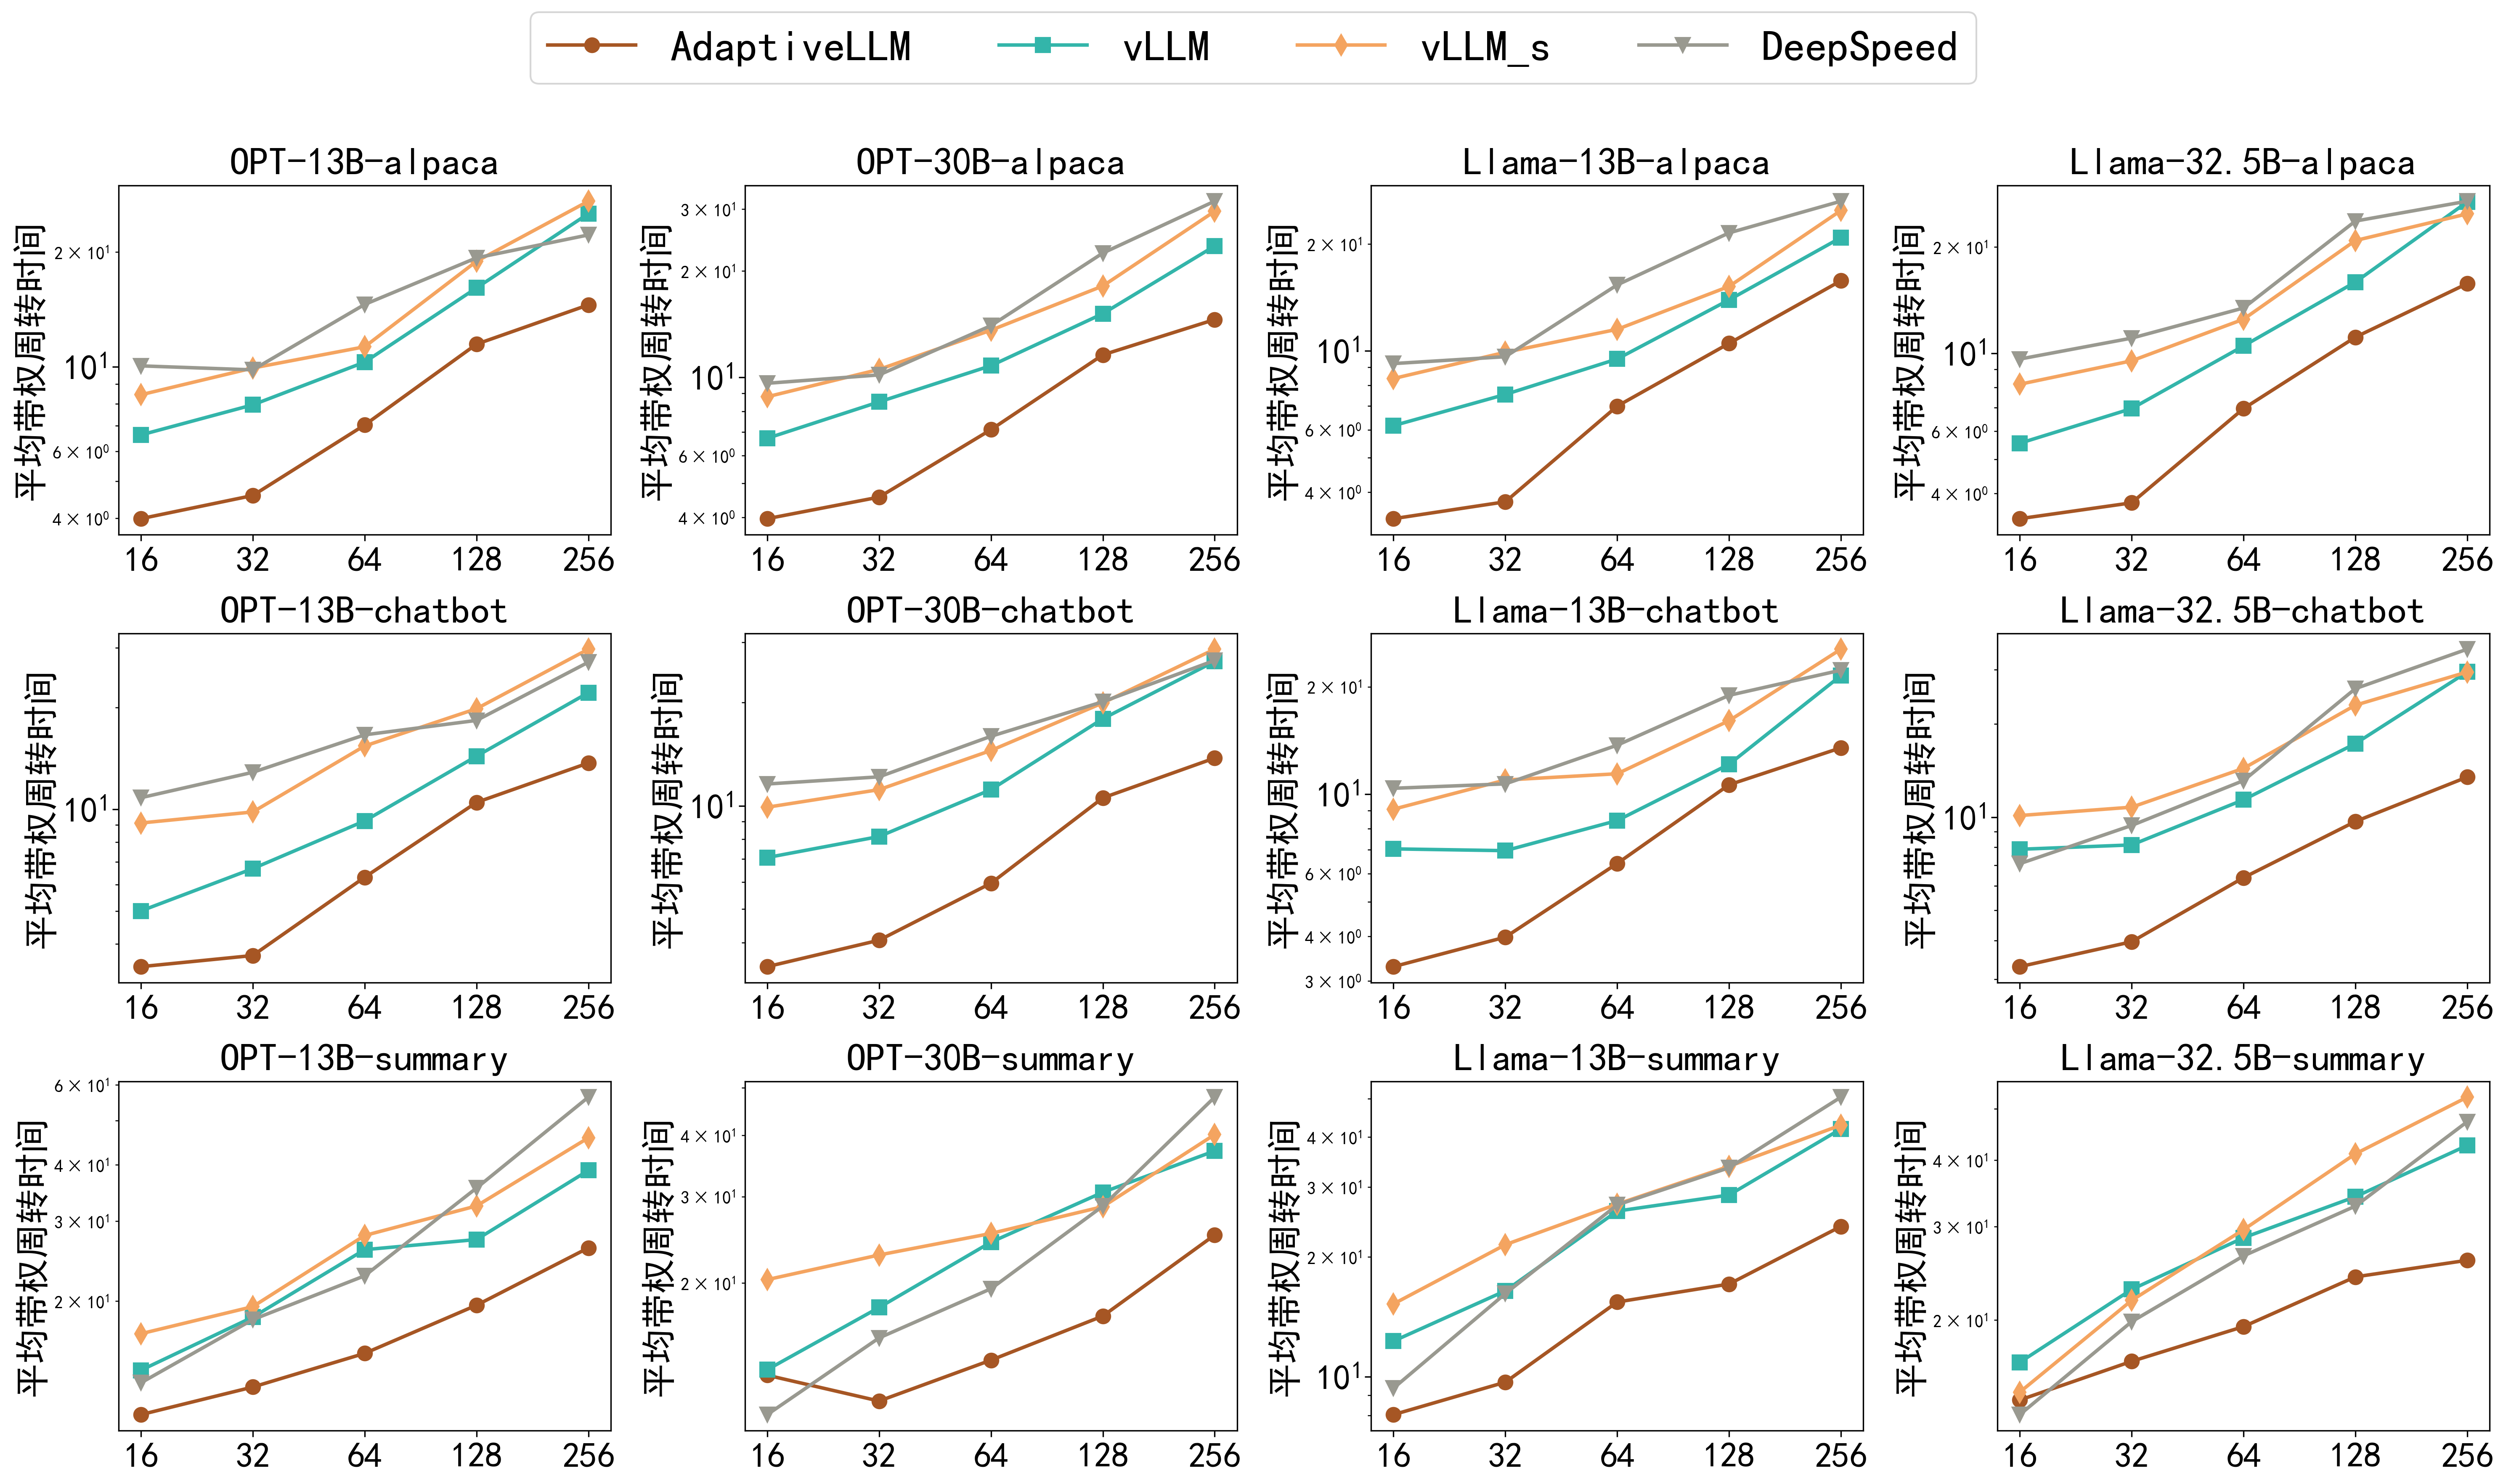
\includegraphics[width=0.9\linewidth]{平均带权周转时间.png}
  \caption{用户请求平均带权周转时间}
  \label{Fig:平均带权周转时间}
\end{figure*}

综上所述,在基于开销感知的内存优化策略下,AdaptiveLLM在GPU内存不足时预测张量交换与张量重算开销,并选择开销较小的内存优化技术执行,进而大幅度提升推理任务整体吞吐率。 

\subsection{实时性测试}

\textcolor{red}{本文选取平均带权周转时间作为实时性测试指标。}用户请求带权周转时间等于客户端响应延迟除以服务器端处理时长,如公式\ref{Eq:Weighted Around Time}所示。对于某一用户请求来说,$finish\_t$是其处理完毕时刻,$send\_t$是其从客户端发送至服务器端的时刻,$sche\_t$是其被AdaptiveLLM初次调度的时刻。平均带权周转时间($\geq 1$)越低,说明用户请求处理过程中的排队时间占比越低。 

\begin{equation}
  \begin{aligned}
    w\_around\_t = \frac{finish\_t - send\_t}{finish\_t - sche\_t}
  \end{aligned}
  \label{Eq:Weighted Around Time}
  \setlength{\abovedisplayskip}{0ex}
  \setlength{\belowdisplayskip}{2ex}
\end{equation}

图\ref{Fig:平均带权周转时间}展示了平均带权周转时间随单序列最大输出长度的变化情况。在相同数据集和LLM配置下,不同框架调度用户请求所产生的平均带权周转时间均随单序列最大输出长度的增加而增加。这是由于随序列长度的增加,有限的GPU内存所能存储的用户请求数量(即批处理大小)下降,导致后续请求的等待时间增加。Summary数据集相比于Alpaca和Chatbot数据集而言,相同条件下用户请求平均带权周转时间更高,但AdaptiveLLM仍能保持较大优势。

表\ref{Table:AdaptiveLLM相对于基准框架的平均带权周转时间缩减比}展示了单序列最大输出长度为64时,AdaptiveLLM相比于三个基准框架的平均带权周转时间缩减比。由表可知,AdapiveLLM的用户请求平均带权周转时间相比于vLLM下降了$20\%\sim50\%$,相比于vLLM$\_$s下降了$30\%\sim60\%$,相比于DeepSpeed-MII下降了$25\%\sim65\%$。

\begin{table}[H]
  \centering
  \caption{AdaptiveLLM相对基准框架的平均带权周转时间缩减比}
  \label{Table:AdaptiveLLM相对于基准框架的平均带权周转时间缩减比}
  \renewcommand{\arraystretch}{1.25}
  \small
  \begin{tabular}{c c c}
    \toprule
    \textbf{LLM} & \textbf{dataset} & \textbf{vLLM/vLLM\_s/DeepSpeed-MII} \\
    \midrule
    OPT-13B	& alpaca & 0.32$\times$/0.38$\times$/0.52$\times$ \\
    OPT-13B	& chatbot & 0.32$\times$/0.59$\times$/0.52$\times$ \\
    OPT-13B	& summary & 0.41$\times$/0.45$\times$/0.33$\times$ \\
    OPT-30B	& alpaca & 0.34$\times$/0.48$\times$/0.49$\times$ \\
    OPT-30B	& chatbot & 0.47$\times$/0.59$\times$/0.63$\times$ \\
    OPT-30B	& summary & 0.42$\times$/0.45$\times$/0.28$\times$ \\
    Llama-13B & alpaca & 0.26$\times$/0.39$\times$/0.54$\times$ \\
    Llama-13B & chatbot & 0.24$\times$/0.44$\times$/0.53$\times$ \\
    Llama-13B & summary & 0.41$\times$/0.43$\times$/0.43$\times$ \\
    Llama-32.5B & alpaca & 0.34$\times$/0.44$\times$/0.48$\times$ \\
    Llama-32.5B & chatbot & 0.44$\times$/0.56$\times$/0.51$\times$ \\
    Llama-32.5B & summary & 0.32$\times$/0.34$\times$/0.26$\times$ \\
    \bottomrule
  \end{tabular}
\end{table}

vLLM基于FCFS策略进行设计,在调度时优先考虑$swapped$队列,只有当$swapped$队列为空时才调度$waiting$队列,使得以交换方式被抢占的用户请求相比于以重算方式被抢占的用户请求,其重调度的优先级更高。结合4.4章节关于vLLM固定式抢占策略的分析可知,一部分用户请求被抢占后能够很快重新调度,而也有一部分用户请求被抢占后进入$waiting$队列的末尾,需要长时间等待。vLLM$\_$s和DeepSpeed同样缺少公平性考虑,因此他们在平均带权周转时间测试中均表现不佳。本文在AdaptiveLLM的设计中引入了基于公平性的用户请求调度策略,使得用户请求从客户端发送至服务器端后能够很快开始处理,不会出现长时间等待现象。

\subsection{预测误差测试}

\subsubsection{张量重算预测误差}

张量重算开销由张量重算开销分析器根据LLM模型层数、LLM模型隐藏维度、以及待处理token总数来预测得到。表\ref{Table:OPT模型单步迭代执行时间预测误差}和表\ref{Table:LLama模型单步迭代执行时间预测误差}分别展示了OPT模型和Llama模型单步推理执行时间的预测效果。OPT执行时间预测任务共有6.4w条训练数据和1.6w条测试数据,结果表明,随机森林回归模型性能最佳,其在拟合2次多项式时能够达到1.76\%的预测误差。Llama执行时间预测任务共有6.8条训练数据和1.7w条测试数据,结果表明,随机森林回归模型同样性能最佳,其在拟合2次多项式时能够达到1.30\%的预测误差。

\begin{table}[H]
  \centering
  \caption{OPT模型单步迭代执行时间预测误差}
  \label{Table:OPT模型单步迭代执行时间预测误差}
  \renewcommand{\arraystretch}{1.25}
  \small
  \begin{tabular}{c c c c c c}
    \toprule
    \textbf{模型-拟合次数} & \textbf{1} & \textbf{2} & \textbf{3} & \textbf{4} & \textbf{5} \\
    \midrule
    线性回归模型 & 46.52 & 46.65 & 28.75 & 11.86 & 9.32 \\ 
    决策树 & 1.81 & 1.81 & 1.81 & 1.81 & 1.81 \\ 
    随机森林 & 1.77 & 1.76 & 1.77 & 1.77 & 1.78 \\ 
    岭回归模型 & 46.52 & 46.37 & 28.45 & 11.51 & 7.36 \\ 
    lasso回归模型 & 40.22 & 25.53 & 27.38 & 26.08 & 25.49 \\ 
    弹性回归模型 & 111.89 & 123.62 & 91.67 & 87.59 & 86.48 \\ 
    梯度提升模型 & 15.57 & 16.05 & 14.80 & 15.09 & 14.68 \\ 
    KNN回归模型 & 2.55 & 2.80 & 2.89 & 3.00 & 3.05 \\ 
    \bottomrule
  \end{tabular}
\end{table}

\begin{table}[H]
  \centering
  \caption{LLama模型单步迭代执行时间预测误差}
  \label{Table:LLama模型单步迭代执行时间预测误差}
  \renewcommand{\arraystretch}{1.25}
  \small
  \begin{tabular}{c c c c c c}
    \toprule
    \textbf{模型-拟合次数} & \textbf{1} & \textbf{2} & \textbf{3} & \textbf{4} & \textbf{5} \\
    \midrule
    线性回归模型 & 76.41 & 69.44 & 39.61 & 12.91 & 9.18 \\ 
    决策树 & 1.33 & 1.32 & 1.33 & 1.33 & 1.34 \\ 
    随机森林 & 1.31 & 1.30 & 1.31 & 1.31 & 1.31 \\ 
    岭回归模型 & 76.41 & 69.01 & 39.18 & 12.73 & 7.72 \\ 
    lasso回归模型 & 69.23 & 33.57 & 34.42 & 35.16 & 31.58  \\ 
    弹性回归模型 & 127.18 & 139.7 & 100.18 & 94.94 & 93.51  \\ 
    梯度提升模型 & 22.42 & 21.97 & 19.42 & 19.99 & 19.38  \\ 
    KNN回归模型 & 2.24 & 2.36 & 2.48 & 2.63 & 2.68 \\ 
    \bottomrule
  \end{tabular}
\end{table}

\subsubsection{张量交换预测误差}

张量交换预测开销由张量交换开销分析器根据用户请求的KV Cache内存占用和GPU-CPU双向传输带宽而计算得到。本文针对模型Llama-13B和Llama-32.5B进行测试,其结果如图\ref{Fig:交换开销预测误差}所示。两个模型换入开销预测的MAPE误差分别为1.5\%和1.1\%,换出开销预测的MAPE误差分别为1.0\%和1.2\%。因此,张量交换开销总预测误差低于4\%。

\begin{figure}[!htbp]
  \centering
  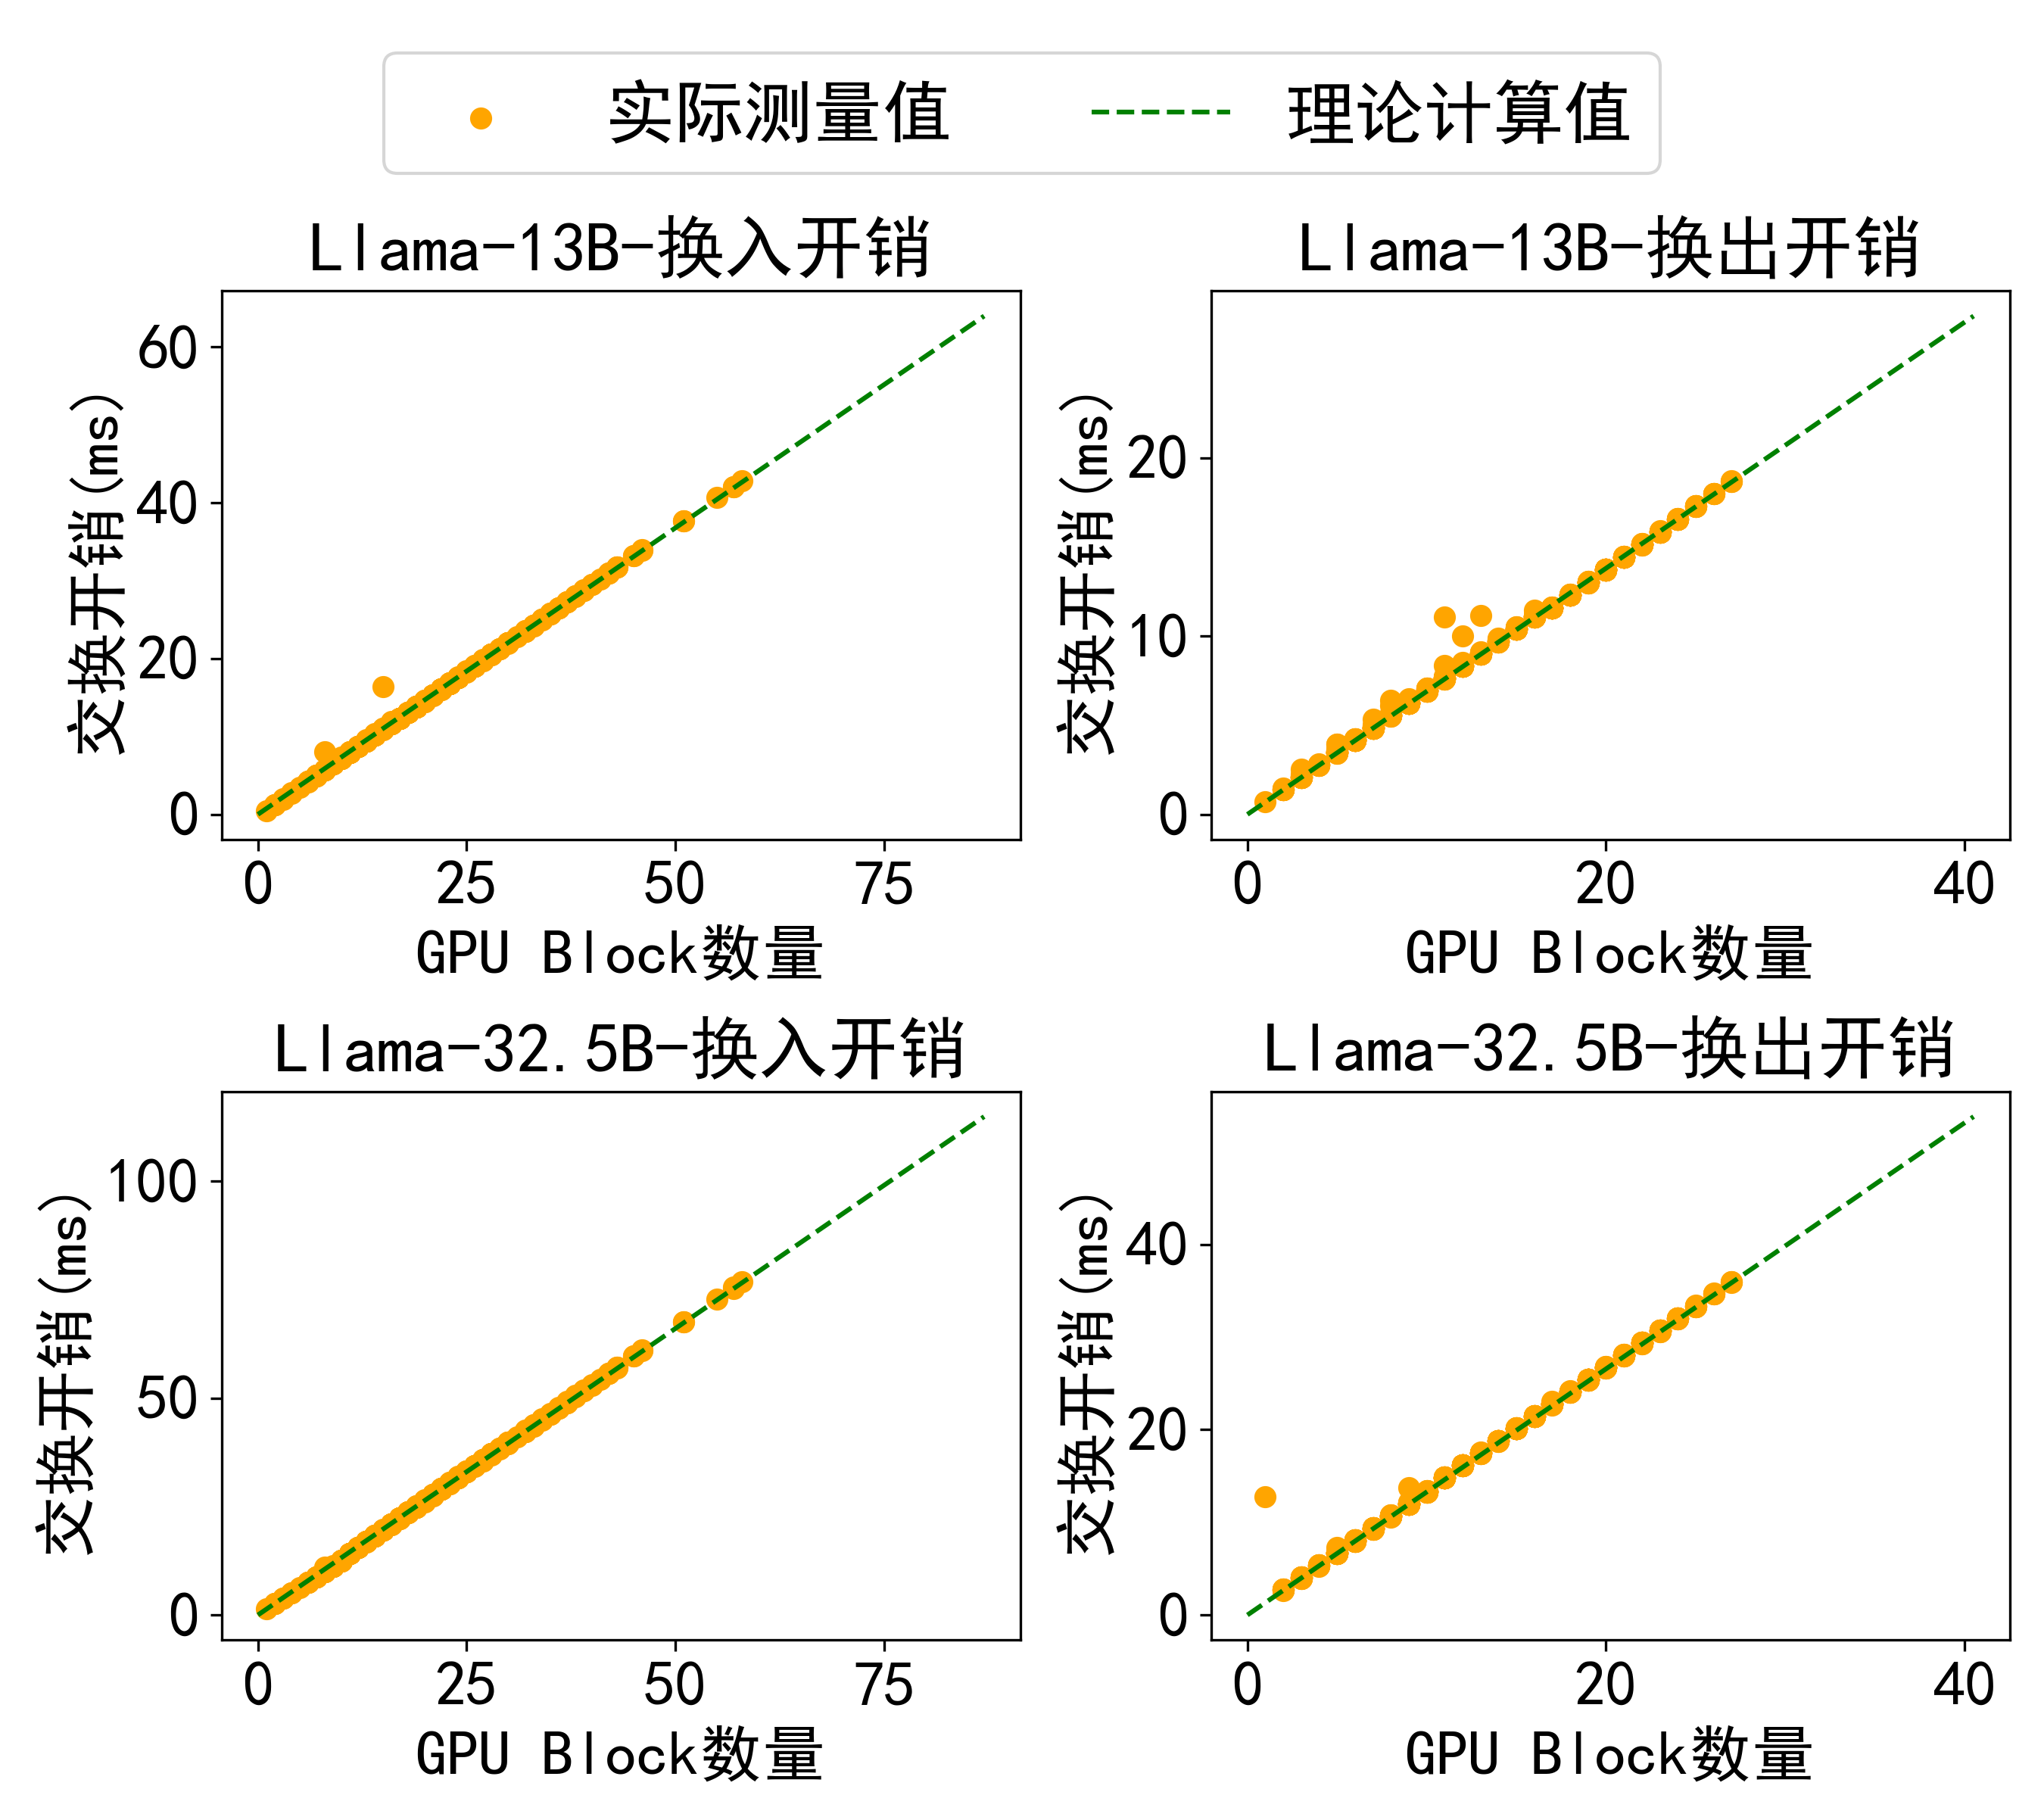
\includegraphics[width=0.88\linewidth]{交换开销预测误差.png}
  \caption{交换开销预测误差}
  \label{Fig:交换开销预测误差}
\end{figure}

\subsection{开销测试}

基于开销感知的内存优化策略在获取张量重算和张量交换开销时,会带来新的预测开销。本文设计如下对照实验获取预测过程的开销:在吞吐率测试过程中,当GPU内存不足时调用开销比较过程,但最终使用vLLM提供的固定式内存优化策略(张量重算)。观察此情景下推理任务的总用时可知,预测开销在推理任务中仅占0.1\%至1\%。

基于公平性的用户请求调度策略也有一定的开销。理论上,该算法的时间复杂度为$O(r^2)$,其中$r$为running队列中用户请求的数量。在实际运行过程中,每次调度的开销在0.2ms左右,总开销在推理任务中仅占0.5\%至1\%。综上所述,AdaptiveLLM引入的两种优化策略所带来的额外开销均可忽略不计。
